\subsection{Training Infrastructure}
\label{subsec::training_infrastructure}

Cosmos 3 leverages a custom infrastructure platform engineered for scaling multimodal foundation-model training. This unified stack coordinates the end-to-end lifecycle for the Reasoner and Generator training. This lifecycle spans raw multimodal sample ingestion, training computation, and persistent checkpointing, and is structured around the stages described below.

\begin{itemize}
    \item \textit{Data loader.} The data loader ingests multimodal samples---images, videos, action, audio, text---at arbitrary native resolutions and aspect ratios.  It applies on-the-fly augmentation (\eg, resizing, spatial cropping, color jitter, and temporal video sub-sampling), tokenizes text conditions, and packs variable-length samples into batches. To hide I/O and pre-processing latency, the loader runs asynchronously in parallel worker processes and prefetches batches onto the device via a pinned-memory staging buffer.

    \item \textit{Distributed training.} Training is parallelized using a combination of Hybrid Sharded Data Parallelism (HSDP) and Context Parallelism (CP). This approach enables scaling to large model sizes and extended input sequence lengths. HSDP shards optimizer states, gradients, and model parameters within each replica group while replicating across groups. CP shards the sequence dimension across devices to handle massive context windows that would otherwise overflow a single GPU's memory capacity. These two strategies compose orthogonally and are dynamically configured per experiment to optimize for the target model size, sequence length, and cluster topology.

    \item \textit{Training loop.} Orchestrated in the style of TorchTitan~\citep{torchtitan}, the training loop executes standard forward, backward, optimization, and learning-rate-scheduling cycles. It natively supports various optimizers (\eg, AdamW and fused variants), schedulers (\eg, cosine with warmup, constant with warmup), and loss functions (cross-entropy loss for Reasoner text and EDM loss for Generator). Also incorporating on-the-fly variational encoders (\eg, the Wan2.2 VAE), the pipeline operates end-to-end on raw multimodal inputs. This design eliminates offline latent-extraction phases and ensures that augmentation, encoding, and training remain in lockstep across runs.

    \item \textit{Checkpoint saving.} Checkpoints are recorded at a configurable cadence and use an asynchronous, off-critical-path persistence mechanism to prevent disk and network I/O from stalling the training loop. Model parameters, optimizer states, and RNG/data-loader state are snapshotted on-device, handed off to a background writer, and serialized to remote storage while training continues uninterrupted.
\end{itemize}

Both Reasoner and Generator are trained with this unified framework, sharing a common trainer, parallelization architecture, optimizers, learning rate schedulers, tokenizers, data loaders, and monitoring utilities.

\subsubsection{Data Loader}
\label{sec::data-loader}

The data loader bridges persistent storage and the training loop: it ingests raw multimodal training data, applies on-the-fly augmentation, and forms the batches consumed by each training step. In Cosmos 3, the data loader is required to satisfy three concurrent requirements:
\begin{itemize}
    \item \textit{Pipeline saturation.} It must stream batches asynchronously to prevent the training loop from stalling or blocking on data I/O.
    \item \textit{Distributed load balancing.} It must emit balanced batches across distributed ranks to minimize cross-rank synchronization stalls and maximize aggregate GPU utilization.
    \item \textit{Distribution fidelity.} It must guarantee that the long-run modality and resolution mixtures strictly adhere to the configured target distribution.
\end{itemize}

In conventional LLM training, all three requirements have well-established remedies.
\begin{itemize}
  \item \textit{Pipeline saturation.} This is achieved by tuning the worker count, prefetch depth, and using pinned-memory staging buffers to overlap host-to-device transfers with compute.
  \item \textit{Load balancing.} This becomes trivial because every sample contributes a fixed number of tokens. Maintaining identical per-rank sample counts guarantees uniform per-rank compute and activation-memory profiles across ranks.
\end{itemize}

However, Cosmos 3 invalidates this recipe along all three axes. Since its joint training corpus spans highly heterogeneous modalities, the per-sample token counts vary by over two orders of magnitude, making token volume the primary driver of compute and memory costs. For example, a single 720p two-second video clip produces more tokens than dozens of short text captions combined. Under this asymmetric workload, allocating equal per-rank sample counts introduces critical systemic inefficiencies: it incurs (a) substantial padding waste due to fixed batch shapes; (b) severe workload imbalance across ranks when modality assignments differ; and (c) at scale NCCL collective timeouts caused by extreme step-time variance.

To address these challenges, the Cosmos 3 data loader is built around four coordinated mechanisms:
(i) \emph{token-budgeted packed sequences}, which bound each rank's per-step workload by a token budget rather than a fixed sample count;
(ii) a \emph{joint data loader}, which multiplexes per-stream loaders into a single unified training batch;
(iii) \emph{rank-synchronous stream selection}, which uses a globally seeded selector to keep all ranks aligned on the same data stream at every step;
and (iv) \emph{look-ahead packing}, which raises the average utilization of the token budget $T_{\max}$.

\paragraph{Token-budgeted packed sequences.}
Rather than fixing the per-step sample count, each rank's workload is bounded by a strict token budget $T_{\max}$. The loader greedily concatenates samples into a single packed sequence---each contributing exactly as many tokens as its serialized form requires, with no padding inserted between samples---until appending the next candidate would exceed $T_{\max}$. By eliminating cross-sample padding, this design bounds the per-step compute cost as a direct and predictable function of $T_{\max}$, isolating the hardware from execution variance induced by a fluctuating modality mix. As a defensive secondary constraint, the per-step sample count is also capped at $N_{\max}$.

\paragraph{Joint data loader.}
Each modality, dataset, or finer-grained data stream is encapsulated in its own loader with a private prefetch buffer that hides storage latency. A \emph{joint data loader} (illustrated in~\cref{fig:joint_dataloader}) multiplexes across these per-stream loaders to assemble a single unified training batch per step, while fully preserving per-stream buffering, prefetching, and observability.

\begin{figure}[t]
    \centering
    \resizebox{\linewidth}{!}{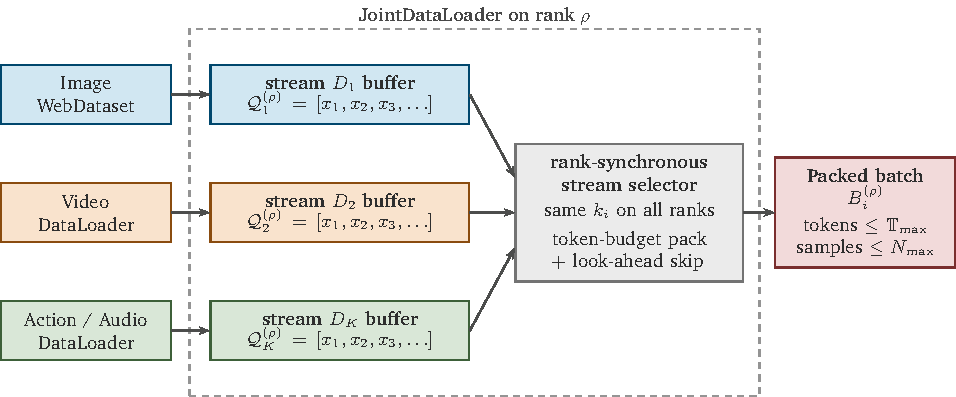
\includegraphics{figures/infrastructure/joint_dataloader.pdf}}
    \captionsetup{justification=raggedright, singlelinecheck=false}
    \caption{\textbf{Overview of the Joint Data-Loader.}
    Stream-specific data-loaders feed local per-stream buffers on each rank.
    At each global iteration, a rank-synchronous selector chooses the same
    stream $k_i$ across distributed ranks. Each rank then greedily packs
    samples from its selected local buffer into $B_i^{(\rho)}$ under token
    and sample-count budgets, using bounded look-ahead to reduce unused
    token capacity.}
    \label{fig:joint_dataloader}
\end{figure}

\paragraph{Rank-synchronous stream selection.}
Foundation-model training typically draws from datasets containing both images and videos at multiple spatial resolutions. Per-sample token counts differ by orders of magnitude across these streams. For example, video samples often carry over $100\times$ more tokens than images, and 720p videos over $10\times$ more than 256p videos. Allowing each rank to choose its stream independently would induce severe workload imbalance under FSDP, with widely divergent attention FLOPs (due to its quadratic complexity) across ranks within a single step. We mitigate this by selecting the active stream via a globally seeded selector keyed on the iteration index, ensuring that all ranks process samples drawn from the same modality and resolution bucket at every step. This eliminates cross-rank variance in compute time and activation memory, while the deterministic, seed-derived selection sequence is bit-exactly reproducible across checkpoints and restarts. Rank-synchronous stream selection improves end-to-end training throughput by $54\%$ over the unsynchronized baseline.

\paragraph{Look-ahead packing.}

Given the stream $k_i$ selected for iteration $i$, the Joint Data-Loader constructs the local batch greedily, appending samples from the head of the stream's buffer until the next candidate would exceed the token budget $\mathbb{T}_{\max}$. Pure greedy packing, however, can leave a non-trivial fraction of the budget unused whenever the next candidate is large enough to overflow but smaller candidates remain available deeper in the buffer---residual capacity that is functionally equivalent to padding and directly proportional to lost throughput. We address this with a bounded look-ahead policy. When a candidate sample exceeds the \emph{total} token budget $\mathbb{T}_{\max}$, the sample is unpackable under the current configuration and is dropped (with a logged warning). When a candidate merely exceeds the \emph{remaining} budget but the batch is already non-empty, the candidate is moved temporarily into a \emph{look-aside buffer}, and the loader continues scanning further into the stream buffer for a smaller sample that fits the residual capacity.

The mechanism is illustrated in \cref{fig:lookahead_dataloader}. In the example, samples $a_1$ and $a_2$ fit into the current batch; $a_3$ exceeds the remaining budget and is diverted to the look-aside buffer; the loader then continues scanning and packs subsequent smaller samples such as $a_4$ and $a_6$. At the end of the iteration, all samples remaining in the look-aside buffer are restored to the head of the stream buffer in their original arrival order, so that look-ahead reduces padding without permanently reordering the stream. To bound the cost of pathological cases---e.g., a stream temporarily dominated by oversized samples---the number of consecutive look-ahead attempts per iteration is capped by a configurable per-stream limit. In production, we use a cap of ten; beyond this value, we observe negligible additional reduction in unused capacity, while the size of the look-aside buffer (and its memory footprint) continues to grow. Overall, look-ahead packing increases the effective sequence length by $8\%$ over the baseline, yielding a corresponding improvement in training throughput.

% =====================================================================
%  cosmos3_palette.tex — Cosmos-3 paper figure colour palette.
%  ─────────────────────────────────────────────────────────────────
%  Requires xcolor (loaded automatically by tikz/pgf).
%
%  IMPORTANT — every non-comment line below ends with `%` so this file
%  is safe to \input inside a horizontal box (e.g. \resizebox{...}{!}{...}).
%  Without those `%`s, each newline would tokenise into a space and
%  leak into the surrounding hbox, padding the figure horizontally.
% =====================================================================
%
%% ── 1. Six base colours ───────────────────────────────────────────
%%
%% Hex values below are the *exact* RGB triples xcolor produces (verified
%% by pixel-sampling a rendered PDF swatch — not back-computed from the
%% mixing formula). Useful to copy-paste into matplotlib / Inkscape /
%% Figma if a collaborator is drawing outside LaTeX.
%%
%% Note: xcolor's `violet` is (0.5, 0, 0.5) → #800080 (a saturated
%% purple). It is NOT the CSS `violet` (#EE82EE) nor "electric violet"
%% (#7F00FF) — three different colours share that English name.
%%
%%   Hue name      Role in the MoT architecture figure              ≈ hex
%%   ------------  ----------------------------------------------- --------
%%   c3OceanBlue   AR-vision tokens, ViT encoder                    #0077B6
%%   c3Blue        AR text tokens, AR LayerNorm / MLP, AR arrows    #0000FF
%%   c3Violet      Action tokens, action encoder                    #800080
%%   c3Rust        Diffusion-vision tokens, VAE encoder             #E58019
%%   c3Orange      Diffusion LN / MLP, generator-tower panel        #FF8000
%%   c3Sage        Audio tokens, audio encoder                      #66A05F
%%
%%   For neutral elements (special tokens, axis arrows, mask grid,
%%   shared-attention slab, ×L bracket) just use xcolor's built-in
%%   `gray` and `black` with !N modifiers, e.g. fill=gray!16, draw=gray!55.
\definecolor{c3OceanBlue}{HTML}{0077B6}%
\colorlet  {c3Blue}   {blue}%
\colorlet  {c3Violet} {violet}%
\colorlet  {c3Orange} {orange}%
\colorlet  {c3Rust}   {orange!60!brown}%                       browner orange
\colorlet  {c3Sage}   {teal!70!green!70!yellow!50!gray}%       muted olive sage
%
%% ── 2. Pre-mixed variants for every base colour ───────────────────
%%
%%   Six standard variants are pre-baked for every base C:
%%
%%     c3{C}Pale    = C!4!white      panel / tower background tint
%%     c3{C}Light   = C!8            extra-pale fill (encoder boxes)
%%     c3{C}Fill    = C!12           standard fill (LN / MLP / blocks)
%%     c3{C}Tok     = C!22           saturated fill (tokens / pills)
%%     c3{C}Soft    = C!50!gray      muted "supporting" outline
%%     c3{C}Dark    = C!50!black     strong outline / arrow / dark text
%%
%%   So a typical "blue token" pairing is:
%%       \node[fill=c3BlueTok, draw=c3BlueDark] {…};
%%   and a typical "blue encoder" pairing is:
%%       \node[fill=c3BlueLight, draw=c3BlueSoft, text=c3BlueDark] {…};
%%
%%   Need a one-off mix that isn't pre-baked?  Use the !N syntax inline:
%%       fill=c3OceanBlue!30!white!85!gray
\providecommand{\cThreeVariants}[1]{%
  \colorlet{c3#1Pale} {c3#1!4!white}%
  \colorlet{c3#1Light}{c3#1!8}%
  \colorlet{c3#1Fill} {c3#1!12}%
  \colorlet{c3#1Tok}  {c3#1!22}%
  \colorlet{c3#1Soft} {c3#1!50!gray}%
  \colorlet{c3#1Dark} {c3#1!50!black}%
}%
\cThreeVariants{Blue}%
\cThreeVariants{OceanBlue}%
\cThreeVariants{Violet}%
\cThreeVariants{Orange}%
\cThreeVariants{Rust}%
\cThreeVariants{Sage}%
%
%% ── 3. Named hue families (semantic palette) ──────────────────────
%%
%% A higher-level naming layer that pairs each light fill with the dark
%% boundary/text colour the MoT figure uses. Useful as a quick lookup
%% for collaborators who think in terms of "audio is Lilac, action is
%% Mint" rather than in mixing recipes.
%%
%% Each pair has the form:
%%     c3{Name}Fill   light tint (box fill)
%%     c3{Name}Dark   saturated colour (border / text)
%%
%% Hex values verified by pixel-sampling the rendered MoT PDF (post
%% action↔audio swap, see tikz_mot_architecture.tex).
%%
%%   Name      Fill recipe          ≈ hex     Dark recipe                ≈ hex     Where in MoT
%%   --------  -------------------  --------  -------------------------  --------  -----------------------------
%%   Sky       c3OceanBlue!18       #D2E7F2   c3OceanBlue!60!black       #00476D   AR-vision tokens
%%   Lavender  c3Blue!12            #E0E0FF   c3Blue!45!black            #000073   AR-text tokens
%%   Mint      c3Sage!25            #D9E7D7   c3Sage!60!black            #3D6039   Action tokens
%%   Lilac     c3Violet!22          #E3C7E3   c3Violet!60!black          #4C004D   Audio tokens
%%   Peach     c3Orange!12          #FFF0E0   c3Orange!78!black          #C76300   DM LN / MLP fill + DM-subseq label
%%   Birch     c3Orange!4!white     #FFFAF5   c3Rust!70!black            #A15911   DM panel background + vid-token border
%%   Gray      gray!16              #ECECEC   black!70                   #4D4D4D   Special tokens (EOS / BOG)
%%   Rose      (literal hex)        #F2DADA   (literal hex)              #7A2E2E   Supplementary accent (not in MoT)
%%
\colorlet  {c3SkyFill}      {c3OceanBlue!18}%
\colorlet  {c3SkyDark}      {c3OceanBlue!60!black}%
\colorlet  {c3LavenderFill} {c3Blue!12}%
\colorlet  {c3LavenderDark} {c3Blue!45!black}%
\colorlet  {c3MintFill}     {c3Sage!25}%
\colorlet  {c3MintDark}     {c3Sage!60!black}%
\colorlet  {c3LilacFill}    {c3Violet!22}%
\colorlet  {c3LilacDark}    {c3Violet!60!black}%
\colorlet  {c3PeachFill}    {c3Orange!12}%
\colorlet  {c3PeachDark}    {c3Orange!78!black}%
\colorlet  {c3BirchFill}    {c3Orange!4!white}%
\colorlet  {c3BirchDark}    {c3Rust!70!black}%
\colorlet  {c3GrayFill}     {gray!16}%
\colorlet  {c3GrayDark}     {black!70}%
\definecolor{c3RoseFill}{HTML}{F2DADA}%
\definecolor{c3RoseDark}{HTML}{7A2E2E}%
%
%% ── 4. Optional parametric shorthand macros ───────────────────────
%%
%%   If you'd rather not memorise the 36 variant names, these macros
%%   take a base-colour NAME and return the right mix:
%%
%%       fill=\cTok{c3Blue}        ≡ fill=c3Blue!22  (same as c3BlueTok)
%%       draw=\cBorder{c3Blue}     ≡ draw=c3Blue!50!black (same as c3BlueDark)
%%       text=\cBorder{c3OceanBlue}≡ text=c3OceanBlue!50!black
%%
%%   The named variants above are usually preferred (more readable,
%%   no macro-expansion gotchas inside \edef), but these are handy
%%   when you're writing a parametric TikZ style.
\providecommand{\cPale}  [1]{#1!4!white}%
\providecommand{\cLight} [1]{#1!8}%
\providecommand{\cFill}  [1]{#1!12}%
\providecommand{\cTok}   [1]{#1!22}%
\providecommand{\cSoft}  [1]{#1!50!gray}%
\providecommand{\cBorder}[1]{#1!50!black}%
%
%% ── 5. Extended qualitative palette (11 hues) ─────────────────────
%%
%% Eleven distinguishable hues for charts that need more categories
%% than the MoT-role hues offer (e.g. multi-slice pies, stacked bars,
%% category legends). Hues are spaced ~30° around the colour wheel
%% and derived from existing cosmos3 base colours wherever possible,
%% so they share family with the rest of the figure set. Three are
%% defined by hex because the cosmos3 base has no equivalent
%% (saturated coral red, magenta-pink, earthy brown); their luminance
%% is tuned to sit alongside the base hues without screaming.
%%
%% Adjacency check: every pair is clearly distinguishable.
%%   • c3Olive (#B3D030, lime ~70°) vs c3Sage (#66A05F, green ~115°)
%%     — different hue and luminance, no green-on-green clash.
%%   • c3Teal (#2E898F, ~180°) vs c3OceanBlue (#0077B6, ~200°)
%%     — close on the wheel but Teal is greener, Ocean is bluer.
%%   • c3Coral (#C95B5B) vs c3Berry (#B04060) vs c3Violet (#800080)
%%     — three reds/pinks/purples, each clearly its own hue.
%%   • c3Cocoa (#8C5523) vs c3Rust (#E58019)
%%     — same hue family, but Cocoa is much darker / lower saturation,
%%       reads as "brown" rather than "rust".
%%
%%   #   Name         Recipe                          ≈ hex     Slot
%%   --  -----------  -----------------------------   --------  --------------
%%   1   c3Coral      HTML C95B5B                     #C95B5B   ~0°  red
%%   2   c3Rust       base                            #E58019   ~30° orange
%%   3   c3Gold       c3Orange!55!yellow              #FFB900   ~45° gold
%%   4   c3Olive      c3Sage!50!yellow                #B3D030   ~70° lime
%%   5   c3Sage       base                            #66A05F   ~115° green
%%   6   c3Teal       c3OceanBlue!55!c3Sage           #2E898F   ~180° teal
%%   7   c3OceanBlue  base                            #0077B6   ~200° blue
%%   8   c3Indigo     c3Blue!65!c3Violet              #2D00D3   ~250° indigo
%%   9   c3Violet     base                            #800080   ~300° violet
%%   10  c3Berry      HTML B04060                     #B04060   ~335° magenta-pink
%%   11  c3Cocoa      HTML 8C5523                     #8C5523   earthy brown
%%
%% Use them in chart order (1→11) for monotonic categorical scales,
%% or pick subsets that visit each colour-wheel sector once. A clean
%% 7-slice pick is e.g. {c3OceanBlue, c3Teal, c3Sage, c3Gold, c3Rust,
%% c3Coral, c3Violet}.
\definecolor{c3Coral} {HTML}{C95B5B}%
\colorlet  {c3Gold}   {c3Orange!55!yellow}%
\colorlet  {c3Olive}  {c3Sage!50!yellow}%
\colorlet  {c3Teal}   {c3OceanBlue!55!c3Sage}%
\colorlet  {c3Indigo} {c3Blue!65!c3Violet}%
\definecolor{c3Berry} {HTML}{B04060}%
\definecolor{c3Cocoa} {HTML}{8C5523}%
%
%% ── 6. Softened chart variants (Tableau-style) ────────────────────
%%
%% The Section-5 hues are full-saturation — fine for the MoT hero plot,
%% but they overpower the page when used as solid fills in a multi-slice
%% pie or stacked bar. This section provides pre-softened versions for
%% chart use: each hue is mixed ~20% toward gray and slightly lightened,
%% bringing the saturation/lightness into Tableau-10 territory while
%% staying in the cosmos3 hue family.
%%
%% Names use prefix `c3Cat` (categorical). Hex values are computed from
%% the recipes shown.
%%
%%   #   Name           Recipe                                    ≈ hex
%%   --  -----------    ------------------------------------      --------
%%   1   c3CatCoral     HTML C36868 (lighter coral)               #C36868
%%   2   c3CatRust      c3Rust!82!gray!97                         #D48431
%%   3   c3CatGold      c3Gold!78!gray!95                         #E4B027
%%   4   c3CatOlive     c3Olive!85!gray!97                        #AEC641
%%   5   c3CatSage      c3Sage!92!gray!97                         #6DA166
%%   6   c3CatTeal      c3Teal!82!gray!95                         #468D92
%%   7   c3CatBlue      c3OceanBlue!80!gray!95                    #2580AF
%%   8   c3CatIndigo    c3Indigo!50!gray!92                       #674FAD
%%   9   c3CatViolet    HTML 9C73A2 (soft mauve, c3Violet doesn't
%%                      desaturate well via gray-mixing alone)    #9C73A2
%%   10  c3CatBerry     c3Berry!85!gray!95                        #AD526D
%%   11  c3CatCocoa     c3Cocoa!90!gray!97                        #8E5E32
%%
%% Use these for any solid-fill categorical chart. Saturated Section-5
%% versions are still available if you need a punchy accent (e.g. one
%% highlighted slice in an otherwise-muted pie).
\definecolor{c3CatCoral} {HTML}{C36868}%
\colorlet  {c3CatRust}   {c3Rust!82!gray!97}%
\colorlet  {c3CatGold}   {c3Gold!78!gray!95}%
\colorlet  {c3CatOlive}  {c3Olive!85!gray!97}%
\colorlet  {c3CatSage}   {c3Sage!92!gray!97}%
\colorlet  {c3CatTeal}   {c3Teal!82!gray!95}%
\colorlet  {c3CatBlue}   {c3OceanBlue!80!gray!95}%
\colorlet  {c3CatIndigo} {c3Indigo!50!gray!92}%
\definecolor{c3CatViolet}{HTML}{9C73A2}%
\colorlet  {c3CatBerry}  {c3Berry!85!gray!95}%
\colorlet  {c3CatCocoa}  {c3Cocoa!90!gray!97}%
\endinput

\newcommand{\packedbox}[1]{%
  \tikz[baseline=(b.base)]{%
    \node[
      draw=c3MintDark,
      fill=c3MintFill,
      text=c3MintDark,
      rounded corners=1.5pt,
      line width=0.7pt,
      minimum width=0.85cm,
      minimum height=0.48cm,
      inner xsep=4pt,
      inner ysep=2pt
    ] (b) {$\mathtt{x}_{#1}^{*}$};%
  }%
}

\newcommand{\skippedbox}[1]{%
  \tikz[baseline=(b.base)]{%
    \node[
      draw=c3RoseDark,
      fill=c3RoseFill,
      text=c3RoseDark,
      rounded corners=1.5pt,
      line width=0.7pt,
      minimum width=0.85cm,
      minimum height=0.48cm,
      inner xsep=4pt,
      inner ysep=2pt
    ] (b) {$\mathtt{x}_{#1}$};%
  }%
}

\newcommand{\boxgap}{\hspace{0.08cm}}

\begin{figure}[t]
\centering
\begin{adjustbox}{max width=0.98\linewidth}
\begin{tabular}{@{}p{4.4cm}p{6.9cm}p{4.1cm}p{7.0cm}@{}}
\textbf{step} &
\textbf{packed (in output\_batch)} &
\textbf{skipped (set aside)} &
\textbf{state} \\
\midrule

\texttt{fetch x1 (fits)}
& \packedbox{1}
&
& $\mathrm{cur}=\tau(x_1)$ \\[0.65em]

\texttt{fetch x2 (fits)}
& \packedbox{1}\boxgap\packedbox{2}
&
& $\mathrm{cur}=\tau(x_1)+\tau(x_2)$ \\[0.65em]

\texttt{fetch x3 (overflow)}
& \packedbox{1}\boxgap\packedbox{2}
& \skippedbox{3}
& $\mathrm{skipped}\leftarrow\{x_3\},\quad \mathrm{lookahead}=1$ \\[0.65em]

\texttt{fetch x4 (fits)}
& \packedbox{1}\boxgap\packedbox{2}\boxgap\packedbox{4}
& \skippedbox{3}
& $\mathrm{cur}\mathrel{+}= \tau(x_4)$ \\[0.65em]

\texttt{fetch x5 (overflow)}
& \packedbox{1}\boxgap\packedbox{2}\boxgap\packedbox{4}
& \skippedbox{3}\boxgap\skippedbox{5}
& $\mathrm{lookahead}=2$ \\[0.65em]

\texttt{fetch x6 (fits, last)}
& \packedbox{1}\boxgap\packedbox{2}\boxgap\packedbox{4}\boxgap\packedbox{6}
& \skippedbox{3}\boxgap\skippedbox{5}
& \texttt{batch done} \\[0.65em]

\texttt{end of iter t}
& \packedbox{1}\boxgap\packedbox{2}\boxgap\packedbox{4}\boxgap\packedbox{6}
& \skippedbox{3}\boxgap\skippedbox{5}
& \texttt{push reversed(skipped)} $\rightarrow$
  \texttt{head: [x3, x5, x7, x8, ...]} \\[0.25em]

\multicolumn{4}{@{}l}{%
  \textcolor{c3MintDark}{\footnotesize $^{*}$ fits in $\mathbb{T}_{\max}$ budget}
}
\end{tabular}
\end{adjustbox}
\captionsetup{justification=raggedright, singlelinecheck=false}
\caption{\textbf{Look-ahead packing in the JointDataLoader.}
The loader greedily scans samples from the selected stream and packs those that fit within the remaining token budget into the current mini-batch (Mint). Samples that exceed the budget are temporarily set aside in a lookaside buffer (Rose), allowing later smaller samples to fill the remaining capacity. At the end of the iteration, skipped samples are returned to the head of the stream buffer in their original arrival order, reducing padding while preserving stream order across iterations.}
\label{fig:lookahead_dataloader}
\end{figure}


\paragraph{Cold-start handling.}
Several of our data streams incur substantial first-batch latency, dominated by worker-process spawning, filesystem metadata caching for newly opened shards, and stream-specific deserialization warm-up. If this latency were paid at the first training step, it would race against the NCCL collective on that step, with a high probability of triggering a watchdog timeout on the slowest rank---particularly at scale, where the maximum over ranks is the relevant statistic. To eliminate this failure mode, the Joint Data-Loader performs an explicit pre-warm stage during construction: it fetches one batch from every stream so that worker pools, file handles, and deserialization caches are fully primed, and then issues a distributed barrier before returning control to the training loop. This guarantees that every rank has paid the cold-start cost before the first forward pass and that the first iteration runs against fully warmed streams.

\paragraph{Observability and integration.}
At every iteration, the Joint Data-Loader emits a structured record of packing statistics to a training-side monitoring callback, which aggregates the per-rank records across the distributed group and logs the result to Weights \& Biases. The reported metrics include the empirical per-stream sampling ratio (compared against the configured target mixture), the number of samples packed per iteration, per-stream buffer occupancy and wait time, the look-ahead saturation rate, and per-iteration token-budget utilization. These metrics expose the failure modes most likely to degrade large-scale training without crashing it so that such issues are surfaced in the training dashboard within minutes of onset rather than discovered later from model behavior.

\subsubsection{Attention Implementation}

As discussed in \cref{sec:cosmos3_mot}, the Mixture-of-Transformers architecture in Cosmos 3 imposes two distinct attention requirements that must coexist within a single forward pass: the Reasoner pathway employs causal attention over the Reasoner tokens only, while the Generator pathway employs bidirectional attention over the concatenation of the Reasoner and the Generator tokens, so that each Generator token can condition on the full context. Naively expressing these heterogeneous masking patterns with general-purpose operators such as FlexAttention produces correct results but underutilizes the hardware: the masking structure is opaque to the kernel, and padding-equivalent work is performed inside otherwise-skipped attention blocks. This degrades tensor-core utilization and inflates memory-bandwidth pressure.

To address this, we co-designed a custom two-way flat attention mechanism that exposes the cross-pathway masking structure directly to a high-performance variable-length attention kernel. \cref{fig:two_way_attention} illustrates the design. The computation is decomposed into two separate kernel invocations. The first handles the Reasoner pathway and is a standard variable-length scaled dot-product attention (SDPA)~\citep{pytorch_varlen_attn} call with a causal mask, operating only on the Reasoner queries, keys, and values. The second handles the Generator pathway and requires the Reasoner and Generator key/value streams to be visible to each Generator query within the same sample, but strictly separated across samples in a packed batch. We achieve this by flattening and interleaving the two token streams at the sample granularity in the order
\[
[R_0, G_0, R_1, G_1, \ldots, R_n, G_n]
\]
where $R_i$ and $G_i$ denote the Reasoner and Generator key/value tokens of sample $i$, respectively. Each Generator query attends bidirectionally over its own sample's $[R_i, G_i]$ block. This formulation expresses the full cross-pathway attention with two variable-length kernel launches per layer, supports both causal and bidirectional masking within one packed representation, eliminates the padding overhead inherent to fixed-length implementations, and yields $22\%$ improvement in end-to-end training throughput compared to a FlexAttention-based baseline for the Cosmos3-Nano model.

\begin{figure*}[t]
  \centering
  \resizebox{\linewidth}{!}{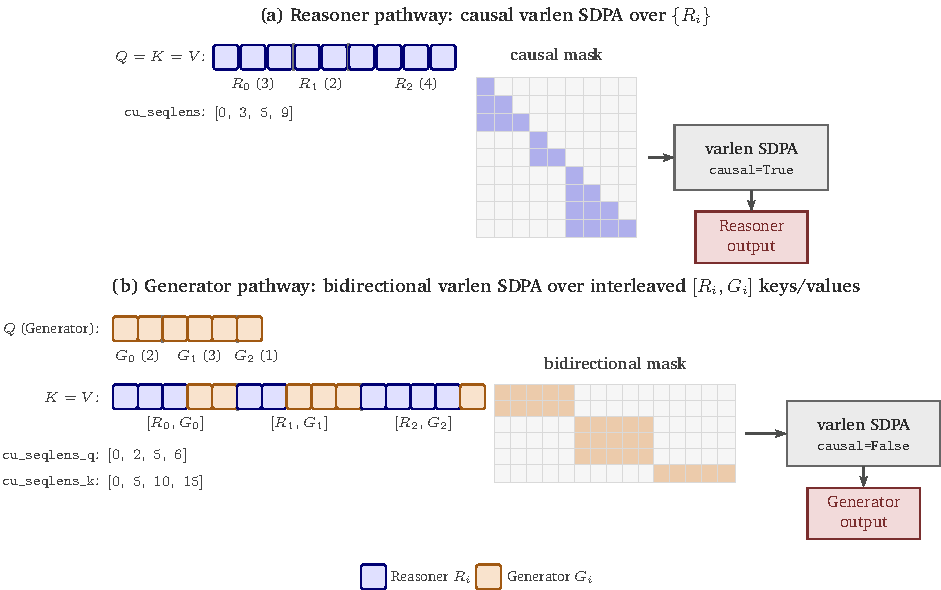
\includegraphics{figures/infrastructure/tikz_two_way_attention.pdf}}
  \captionsetup{justification=raggedright, singlelinecheck=false}
  \caption{\textbf{Two-way flat attention.} Each pathway is implemented as a single
  variable-length SDPA call. \textbf{(a)}~The Reasoner pathway uses a standard causal
  \texttt{varlen} call on the packed Reasoner tokens, producing a block-diagonal
  causal mask. \textbf{(b)}~The Generator pathway packs Generator queries separately
  from the interleaved key/value stream $[R_0, G_0, R_1, G_1, \ldots, R_n, G_n]$. The
  resulting mask is block-diagonal but rectangular within each block, so that each
  Generator query attends bidirectionally over its own sample's $[R_i, G_i]$ context
  without crossing sample boundaries. The example uses three packed samples with
  $(|R_i|, |G_i|) = (3, 2),\,(2, 3),\,(4, 1)$.}
  \label{fig:two_way_attention}
  \vspace{-0.5\baselineskip}
\end{figure*}


The variable-length attention backend is selected per platform to match the most performant and numerically validated implementation available on the target hardware. On Hopper-class GPUs (H100, H200), we use FlashAttention-3~\citep{flash3}, which exploits the WGMMA instructions and TMA-based asynchronous data movement of the Hopper architecture to deliver near-peak attention throughput. On Blackwell-class GPUs (GB200), we use NATTEN~\citep{natten}, whose variable-length kernels are built on the CUTLASS template library and are specifically tuned for the fifth-generation tensor cores and updated memory hierarchy of Blackwell (SM100/SM103). Both backends are accessed through a common dispatch interface, so the choice of kernel is transparent to the rest of the training stack and can be revisited as new backends mature.

\subsubsection{Distributed Training}

Cosmos 3 Reasoner and Generator are trained separately with a distributed-training stack that combines Hybrid Sharded Data Parallelism (HSDP) with Context Parallelism (CP). HSDP shards model parameters, gradients, and optimizer states within each replica group while replicating across groups, which trades a modest amount of intra-group communication for the memory headroom required to train multi-billion-parameter models on commodity per-GPU memory budgets. CP, in contrast, addresses a different bottleneck: per-sequence activation memory, which scales linearly with context length and would otherwise force a hard upper bound on the trainable sequence size. The two strategies compose orthogonally, and the (HSDP-degree, CP-degree) configuration is chosen per experiment to fit the target model size, sequence length, and cluster topology.

\paragraph{Context parallelism via the Ulysses scheme.}

For CP, we adopt the Ulysses scheme~\citep{deepspeed_ulysses}, which partitions the input sequence along the token dimension across CP-rank devices outside of attention and employs two all-to-all collectives per attention layer to transition between sharding axes. The first collective redistributes the Q/K/V activations from the sequence dimension to the attention-head dimension, so that each rank holds the complete sequence for a disjoint subset of heads and can execute attention locally without further cross-rank communication; the second collective restores the original sequence-sharded layout on the attention output.

The scheme integrates cleanly with sequence packing (described in~\cref{sec::data-loader}) and the two-way attention mechanism. The flattening and interleaving of the Reasoner and Generator key/value streams for the bidirectional attention operation is deferred until after the head-axis redistribution, at which point each rank already holds the full sequence for its assigned heads and can perform the concatenation locally. The same variable-length attention kernels are therefore reused unchanged inside CP, with no need for CP-specific kernel variants. The maximum CP degree supported by this implementation is bounded by the number of query heads in the model---32 for Cosmos3-Nano and 64 for Cosmos3-Super---which we find to be a non-restrictive limit in practice given the context lengths and per-GPU memory budgets targeted by Cosmos 3.

\paragraph{Why not ring attention?}

We considered implementing CP via ring attention as an alternative, but found it substantially less attractive in our setting. Ring attention would require materializing a single packed sequence containing the interleaved Reasoner and Generator tokens before sharding it across CP ranks, in order to expose a contiguous K/V stream to the ring schedule. This precludes the independent sharding of the two pathways that Ulysses naturally permits, and complicates the construction of the per-sample bidirectional/causal masks under the rotating ring schedule. Combined with the favorable bandwidth profile of all-to-all on NVLink-connected nodes, these factors led us to adopt Ulysses as the CP strategy for Cosmos 3.

\subsubsection{Selective Activation Checkpointing}

Computing the backward pass of a transformer requires the intermediate activations produced during the forward pass to be available, but materializing all of them simultaneously in GPU memory is prohibitive at the model sizes and context lengths targeted by Cosmos 3. The standard mitigation is activation checkpointing~\citep{sac}: the forward pass stores only a sparse set of ``anchor'' activations and discards the rest, and the discarded tensors are recomputed during the backward pass by re-running the corresponding forward subgraph from the nearest saved anchor. The default policy stores only the inputs of each transformer block and recomputes everything inside the block on demand; this minimizes activation memory but introduces an additional forward pass during backward, inflating per-step FLOPs by roughly $33\%$ and reducing end-to-end training throughput accordingly.

To reduce this recomputation overhead while staying within the activation-memory budget, we apply Selective Activation Checkpointing (SAC), in which a curated subset of intermediate tensors is additionally retained in memory rather than recomputed. The selection is guided by a simple cost-benefit heuristic: rank candidate operations by their FLOPs-to-memory ratio---i.e., the recomputation cost saved per byte of activation memory committed---and materialize those with the highest ratio first, until the activation-memory budget is exhausted. For Cosmos 3, attention outputs are by far the dominant beneficiary of this policy. Attention recomputation is expensive because its cost scales quadratically with sequence length, yet the attention output tensor itself is comparatively small (linear in sequence length and hidden size), making it the operation with the highest FLOPs-to-memory ratio. Users can additionally configure custom save sets through regular-expression patterns over operation names, which we use to retain a small number of secondary tensors when the residual activation-memory headroom permits.

In our measurements, applying SAC with attention outputs materialized yields a $13\%$ improvement in end-to-end training throughput for Cosmos3-Nano at a per-batch token budget of $74{,}000$ tokens, with no change in numerical results.

\subsubsection{Torch Compile for Transformer Blocks}

We apply \texttt{torch.compile} with \texttt{fullgraph=True} and \texttt{dynamic=True} across the training graph. The \texttt{fullgraph} mode eliminates CPU overheads and enables operator fusion, while \texttt{dynamic=True} handles the variable sequence lengths arising from mixed-modality batches---where, for example, Generator pathway tokens are substantially longer than those of image batches across iterations. Torch compile improves training throughput by $41\%$ for Cosmos3-Nano Generator training.

\subsubsection{Video Tokenizer}

Cosmos 3 training requires decoded video frames to be tokenized on-the-fly into latent representations by a video VAE: Wan2.2~\citep{wan2pt2} in our configurations. In the initial implementation, we observed that the tokenizer occupied a disproportionate fraction of each training step---dominating the forward pass for the smaller Cosmos3-Edge and Cosmos3-Nano models. In such models, the transformer compute is small enough that the VAE is not amortized by the rest of the step. Because the tokenizer sits on the critical path between the data loader and the training loop, any latency it introduces directly degrades training throughput. We therefore implemented a series of targeted optimizations that, together, reduce the tokenizer's wall-clock contribution significantly.

\paragraph{Chunked encoding.}

The Wan2.2 causal tokenizer encodes a 1-frame ``prime'' chunk followed by groups of 4 pixel frames per latent chunk; the default per-call granularity is one latent chunk (\ie, 4 frames after the prime). This default leaves the GPU substantially under-utilized for the spatial resolutions used in training, because each kernel launch operates on too little work to saturate the tensor cores. We instead invoke the encoder on a configurable number of pixel frames per call, trading additional activation memory for higher arithmetic intensity per launch. The optimal chunk size is resolution-dependent. At higher spatial resolutions, each frame already consumes substantial memory, so fewer frames per call are admissible before triggering OOMs, whereas at lower resolutions, much larger chunks are feasible and beneficial. We empirically determined the following operating points on our training hardware: 68 frames for 256p, 24 frames for 480p, and 12 frames for 720p. These configurations push the encoder onto the compute-bound side of the roofline curve while staying well under per-GPU memory budgets, yielding the bulk of the per-step speedup.

\paragraph{Ahead-of-time compilation.}

% =====================================================================
%  cosmos3_palette.tex — Cosmos-3 paper figure colour palette.
%  ─────────────────────────────────────────────────────────────────
%  Requires xcolor (loaded automatically by tikz/pgf).
%
%  IMPORTANT — every non-comment line below ends with `%` so this file
%  is safe to \input inside a horizontal box (e.g. \resizebox{...}{!}{...}).
%  Without those `%`s, each newline would tokenise into a space and
%  leak into the surrounding hbox, padding the figure horizontally.
% =====================================================================
%
%% ── 1. Six base colours ───────────────────────────────────────────
%%
%% Hex values below are the *exact* RGB triples xcolor produces (verified
%% by pixel-sampling a rendered PDF swatch — not back-computed from the
%% mixing formula). Useful to copy-paste into matplotlib / Inkscape /
%% Figma if a collaborator is drawing outside LaTeX.
%%
%% Note: xcolor's `violet` is (0.5, 0, 0.5) → #800080 (a saturated
%% purple). It is NOT the CSS `violet` (#EE82EE) nor "electric violet"
%% (#7F00FF) — three different colours share that English name.
%%
%%   Hue name      Role in the MoT architecture figure              ≈ hex
%%   ------------  ----------------------------------------------- --------
%%   c3OceanBlue   AR-vision tokens, ViT encoder                    #0077B6
%%   c3Blue        AR text tokens, AR LayerNorm / MLP, AR arrows    #0000FF
%%   c3Violet      Action tokens, action encoder                    #800080
%%   c3Rust        Diffusion-vision tokens, VAE encoder             #E58019
%%   c3Orange      Diffusion LN / MLP, generator-tower panel        #FF8000
%%   c3Sage        Audio tokens, audio encoder                      #66A05F
%%
%%   For neutral elements (special tokens, axis arrows, mask grid,
%%   shared-attention slab, ×L bracket) just use xcolor's built-in
%%   `gray` and `black` with !N modifiers, e.g. fill=gray!16, draw=gray!55.
\definecolor{c3OceanBlue}{HTML}{0077B6}%
\colorlet  {c3Blue}   {blue}%
\colorlet  {c3Violet} {violet}%
\colorlet  {c3Orange} {orange}%
\colorlet  {c3Rust}   {orange!60!brown}%                       browner orange
\colorlet  {c3Sage}   {teal!70!green!70!yellow!50!gray}%       muted olive sage
%
%% ── 2. Pre-mixed variants for every base colour ───────────────────
%%
%%   Six standard variants are pre-baked for every base C:
%%
%%     c3{C}Pale    = C!4!white      panel / tower background tint
%%     c3{C}Light   = C!8            extra-pale fill (encoder boxes)
%%     c3{C}Fill    = C!12           standard fill (LN / MLP / blocks)
%%     c3{C}Tok     = C!22           saturated fill (tokens / pills)
%%     c3{C}Soft    = C!50!gray      muted "supporting" outline
%%     c3{C}Dark    = C!50!black     strong outline / arrow / dark text
%%
%%   So a typical "blue token" pairing is:
%%       \node[fill=c3BlueTok, draw=c3BlueDark] {…};
%%   and a typical "blue encoder" pairing is:
%%       \node[fill=c3BlueLight, draw=c3BlueSoft, text=c3BlueDark] {…};
%%
%%   Need a one-off mix that isn't pre-baked?  Use the !N syntax inline:
%%       fill=c3OceanBlue!30!white!85!gray
\providecommand{\cThreeVariants}[1]{%
  \colorlet{c3#1Pale} {c3#1!4!white}%
  \colorlet{c3#1Light}{c3#1!8}%
  \colorlet{c3#1Fill} {c3#1!12}%
  \colorlet{c3#1Tok}  {c3#1!22}%
  \colorlet{c3#1Soft} {c3#1!50!gray}%
  \colorlet{c3#1Dark} {c3#1!50!black}%
}%
\cThreeVariants{Blue}%
\cThreeVariants{OceanBlue}%
\cThreeVariants{Violet}%
\cThreeVariants{Orange}%
\cThreeVariants{Rust}%
\cThreeVariants{Sage}%
%
%% ── 3. Named hue families (semantic palette) ──────────────────────
%%
%% A higher-level naming layer that pairs each light fill with the dark
%% boundary/text colour the MoT figure uses. Useful as a quick lookup
%% for collaborators who think in terms of "audio is Lilac, action is
%% Mint" rather than in mixing recipes.
%%
%% Each pair has the form:
%%     c3{Name}Fill   light tint (box fill)
%%     c3{Name}Dark   saturated colour (border / text)
%%
%% Hex values verified by pixel-sampling the rendered MoT PDF (post
%% action↔audio swap, see tikz_mot_architecture.tex).
%%
%%   Name      Fill recipe          ≈ hex     Dark recipe                ≈ hex     Where in MoT
%%   --------  -------------------  --------  -------------------------  --------  -----------------------------
%%   Sky       c3OceanBlue!18       #D2E7F2   c3OceanBlue!60!black       #00476D   AR-vision tokens
%%   Lavender  c3Blue!12            #E0E0FF   c3Blue!45!black            #000073   AR-text tokens
%%   Mint      c3Sage!25            #D9E7D7   c3Sage!60!black            #3D6039   Action tokens
%%   Lilac     c3Violet!22          #E3C7E3   c3Violet!60!black          #4C004D   Audio tokens
%%   Peach     c3Orange!12          #FFF0E0   c3Orange!78!black          #C76300   DM LN / MLP fill + DM-subseq label
%%   Birch     c3Orange!4!white     #FFFAF5   c3Rust!70!black            #A15911   DM panel background + vid-token border
%%   Gray      gray!16              #ECECEC   black!70                   #4D4D4D   Special tokens (EOS / BOG)
%%   Rose      (literal hex)        #F2DADA   (literal hex)              #7A2E2E   Supplementary accent (not in MoT)
%%
\colorlet  {c3SkyFill}      {c3OceanBlue!18}%
\colorlet  {c3SkyDark}      {c3OceanBlue!60!black}%
\colorlet  {c3LavenderFill} {c3Blue!12}%
\colorlet  {c3LavenderDark} {c3Blue!45!black}%
\colorlet  {c3MintFill}     {c3Sage!25}%
\colorlet  {c3MintDark}     {c3Sage!60!black}%
\colorlet  {c3LilacFill}    {c3Violet!22}%
\colorlet  {c3LilacDark}    {c3Violet!60!black}%
\colorlet  {c3PeachFill}    {c3Orange!12}%
\colorlet  {c3PeachDark}    {c3Orange!78!black}%
\colorlet  {c3BirchFill}    {c3Orange!4!white}%
\colorlet  {c3BirchDark}    {c3Rust!70!black}%
\colorlet  {c3GrayFill}     {gray!16}%
\colorlet  {c3GrayDark}     {black!70}%
\definecolor{c3RoseFill}{HTML}{F2DADA}%
\definecolor{c3RoseDark}{HTML}{7A2E2E}%
%
%% ── 4. Optional parametric shorthand macros ───────────────────────
%%
%%   If you'd rather not memorise the 36 variant names, these macros
%%   take a base-colour NAME and return the right mix:
%%
%%       fill=\cTok{c3Blue}        ≡ fill=c3Blue!22  (same as c3BlueTok)
%%       draw=\cBorder{c3Blue}     ≡ draw=c3Blue!50!black (same as c3BlueDark)
%%       text=\cBorder{c3OceanBlue}≡ text=c3OceanBlue!50!black
%%
%%   The named variants above are usually preferred (more readable,
%%   no macro-expansion gotchas inside \edef), but these are handy
%%   when you're writing a parametric TikZ style.
\providecommand{\cPale}  [1]{#1!4!white}%
\providecommand{\cLight} [1]{#1!8}%
\providecommand{\cFill}  [1]{#1!12}%
\providecommand{\cTok}   [1]{#1!22}%
\providecommand{\cSoft}  [1]{#1!50!gray}%
\providecommand{\cBorder}[1]{#1!50!black}%
%
%% ── 5. Extended qualitative palette (11 hues) ─────────────────────
%%
%% Eleven distinguishable hues for charts that need more categories
%% than the MoT-role hues offer (e.g. multi-slice pies, stacked bars,
%% category legends). Hues are spaced ~30° around the colour wheel
%% and derived from existing cosmos3 base colours wherever possible,
%% so they share family with the rest of the figure set. Three are
%% defined by hex because the cosmos3 base has no equivalent
%% (saturated coral red, magenta-pink, earthy brown); their luminance
%% is tuned to sit alongside the base hues without screaming.
%%
%% Adjacency check: every pair is clearly distinguishable.
%%   • c3Olive (#B3D030, lime ~70°) vs c3Sage (#66A05F, green ~115°)
%%     — different hue and luminance, no green-on-green clash.
%%   • c3Teal (#2E898F, ~180°) vs c3OceanBlue (#0077B6, ~200°)
%%     — close on the wheel but Teal is greener, Ocean is bluer.
%%   • c3Coral (#C95B5B) vs c3Berry (#B04060) vs c3Violet (#800080)
%%     — three reds/pinks/purples, each clearly its own hue.
%%   • c3Cocoa (#8C5523) vs c3Rust (#E58019)
%%     — same hue family, but Cocoa is much darker / lower saturation,
%%       reads as "brown" rather than "rust".
%%
%%   #   Name         Recipe                          ≈ hex     Slot
%%   --  -----------  -----------------------------   --------  --------------
%%   1   c3Coral      HTML C95B5B                     #C95B5B   ~0°  red
%%   2   c3Rust       base                            #E58019   ~30° orange
%%   3   c3Gold       c3Orange!55!yellow              #FFB900   ~45° gold
%%   4   c3Olive      c3Sage!50!yellow                #B3D030   ~70° lime
%%   5   c3Sage       base                            #66A05F   ~115° green
%%   6   c3Teal       c3OceanBlue!55!c3Sage           #2E898F   ~180° teal
%%   7   c3OceanBlue  base                            #0077B6   ~200° blue
%%   8   c3Indigo     c3Blue!65!c3Violet              #2D00D3   ~250° indigo
%%   9   c3Violet     base                            #800080   ~300° violet
%%   10  c3Berry      HTML B04060                     #B04060   ~335° magenta-pink
%%   11  c3Cocoa      HTML 8C5523                     #8C5523   earthy brown
%%
%% Use them in chart order (1→11) for monotonic categorical scales,
%% or pick subsets that visit each colour-wheel sector once. A clean
%% 7-slice pick is e.g. {c3OceanBlue, c3Teal, c3Sage, c3Gold, c3Rust,
%% c3Coral, c3Violet}.
\definecolor{c3Coral} {HTML}{C95B5B}%
\colorlet  {c3Gold}   {c3Orange!55!yellow}%
\colorlet  {c3Olive}  {c3Sage!50!yellow}%
\colorlet  {c3Teal}   {c3OceanBlue!55!c3Sage}%
\colorlet  {c3Indigo} {c3Blue!65!c3Violet}%
\definecolor{c3Berry} {HTML}{B04060}%
\definecolor{c3Cocoa} {HTML}{8C5523}%
%
%% ── 6. Softened chart variants (Tableau-style) ────────────────────
%%
%% The Section-5 hues are full-saturation — fine for the MoT hero plot,
%% but they overpower the page when used as solid fills in a multi-slice
%% pie or stacked bar. This section provides pre-softened versions for
%% chart use: each hue is mixed ~20% toward gray and slightly lightened,
%% bringing the saturation/lightness into Tableau-10 territory while
%% staying in the cosmos3 hue family.
%%
%% Names use prefix `c3Cat` (categorical). Hex values are computed from
%% the recipes shown.
%%
%%   #   Name           Recipe                                    ≈ hex
%%   --  -----------    ------------------------------------      --------
%%   1   c3CatCoral     HTML C36868 (lighter coral)               #C36868
%%   2   c3CatRust      c3Rust!82!gray!97                         #D48431
%%   3   c3CatGold      c3Gold!78!gray!95                         #E4B027
%%   4   c3CatOlive     c3Olive!85!gray!97                        #AEC641
%%   5   c3CatSage      c3Sage!92!gray!97                         #6DA166
%%   6   c3CatTeal      c3Teal!82!gray!95                         #468D92
%%   7   c3CatBlue      c3OceanBlue!80!gray!95                    #2580AF
%%   8   c3CatIndigo    c3Indigo!50!gray!92                       #674FAD
%%   9   c3CatViolet    HTML 9C73A2 (soft mauve, c3Violet doesn't
%%                      desaturate well via gray-mixing alone)    #9C73A2
%%   10  c3CatBerry     c3Berry!85!gray!95                        #AD526D
%%   11  c3CatCocoa     c3Cocoa!90!gray!97                        #8E5E32
%%
%% Use these for any solid-fill categorical chart. Saturated Section-5
%% versions are still available if you need a punchy accent (e.g. one
%% highlighted slice in an otherwise-muted pie).
\definecolor{c3CatCoral} {HTML}{C36868}%
\colorlet  {c3CatRust}   {c3Rust!82!gray!97}%
\colorlet  {c3CatGold}   {c3Gold!78!gray!95}%
\colorlet  {c3CatOlive}  {c3Olive!85!gray!97}%
\colorlet  {c3CatSage}   {c3Sage!92!gray!97}%
\colorlet  {c3CatTeal}   {c3Teal!82!gray!95}%
\colorlet  {c3CatBlue}   {c3OceanBlue!80!gray!95}%
\colorlet  {c3CatIndigo} {c3Indigo!50!gray!92}%
\definecolor{c3CatViolet}{HTML}{9C73A2}%
\colorlet  {c3CatBerry}  {c3Berry!85!gray!95}%
\colorlet  {c3CatCocoa}  {c3Cocoa!90!gray!97}%
\endinput

\begin{figure}[t]
\centering
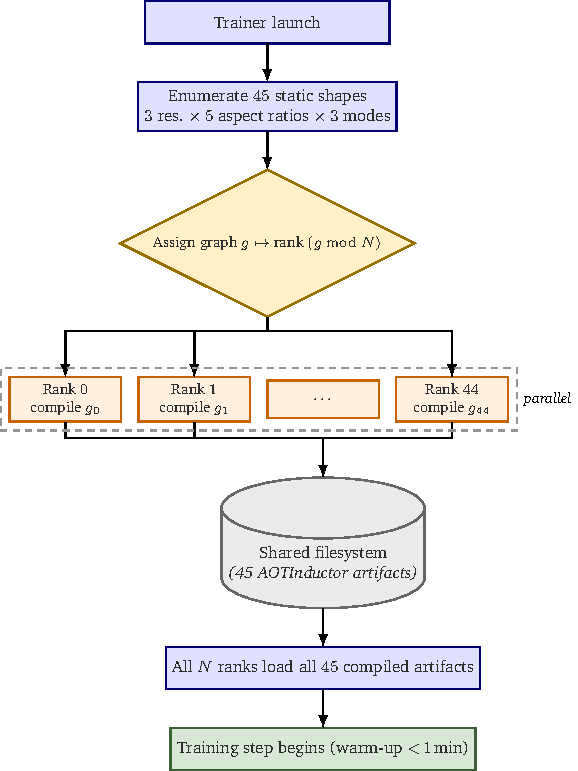
\includegraphics[width=0.58719\linewidth]{figures/infrastructure/aoti_compile_figure.pdf}
\captionsetup{justification=raggedright, singlelinecheck=false}
\caption{\textbf{Sharded AOT compilation of the Wan2.2 tokenizer.} The $45$ static-shape graphs
arising from $\{3\text{ resolutions}\} \times \{5\text{ aspect ratios}\} \times
\{3\text{ tokenizer call modes}\}$ are partitioned across ranks; each
rank performs compilation on its assigned graph(s), writes the compiled
artifact to a shared filesystem, and loads the full set of artifacts
before training begins. Warm-up time drops from $\sim\!15$\,min (serial) to
$<\!1$\,min (sharded).}
\label{fig:aoti_sharded_compile}
\vspace{-0.5\baselineskip}
\end{figure}


On top of chunked encoding, we use \texttt{torch.compile} on the tokenizer, which delivers an additional $52\%$ reduction in encode latency by fusing pointwise operations and selecting optimized kernel schedules for the encoder's convolution and attention blocks. Maximizing throughput requires static input shapes, so the encoder is compiled separately for each shape it may be invoked with. Cosmos 3 training spans three spatial resolutions ($256\text{p}$, $480\text{p}$, $720\text{p}$) and five aspect ratios per resolution. Within each (resolution, aspect-ratio) combination, the causal tokenizer is called in two modes: prime-chunk encoding and chunked encoding with cache sizes of $1$ and $2$. This yields $3 \times 5 \times 3 = 45$ distinct graphs that must be compiled before training can begin. Compiling all $45$ graphs serially on every rank inflated trainer startup by roughly $15$ minutes.

To eliminate this overhead, we shard the compilation across data-parallel ranks using AOTInductor~\citep{pytorch_aot_inductor} as shown in \cref{fig:aoti_sharded_compile}, which performs ahead-of-time compilation and serializes the resulting kernels and host code to disk. With at least $45$ ranks (which is satisfied by all of our training configurations), each rank compiles exactly one graph; the compiled artifacts are written to a shared filesystem, after which every rank loads the full set of $45$ graphs from disk. This reduces the warm-up overhead to under one minute. To accommodate videos with arbitrary frame counts under static-shape compilation, each input clip is right-padded to the next multiple of the configured encode-chunk size prior to encoding, and the resulting latent tensor is cropped along the temporal axis to the exact expected sequence length before being consumed by the model.

\paragraph{Specialization to known frame counts.}

For datasets in which the per-clip frame count is fixed and known a priori---for example, robot action datasets, where every episode contributes a clip of identical length---we specialize the compilation to the exact tensor shapes that arise at runtime, bypassing the padding-and-crop fallback used in the general case. This eliminates the padded-tail compute, removes the corresponding latent-cropping step, and yields a small but consistent additional throughput improvement on such datasets.

\subsubsection{Checkpointing}

To eliminate save-induced stalls, checkpointing is fully overlapped with training. Following Torchtitan~\citep{torchtitan}, checkpoint writes are routed through a dedicated Gloo process group rather than the NCCL communicator carrying training collectives, isolating I/O traffic from GPU-side communication. This asynchronous design hides the highly variable object-store write latencies and removes nearly all save-time overhead, at the cost of a modest increase in host memory. \cref{tab:cosmos3_checkpointing} quantifies the resulting benefit: relative to synchronous checkpointing at a 30-minute interval, asynchronous checkpointing reduces end-to-end training time by $4\%$ for Cosmos3-Nano and $9\%$ for Cosmos3-Super.

\begin{table}[t]
    \centering
    \caption{\textbf{Benefits of asynchronous checkpointing.} Compared with synchronous checkpointing at a 30-minute interval, asynchronous checkpointing reduces end-to-end training time by $4\%$ and $9\%$ for \textbf{Cosmos3-Nano} and \textbf{Cosmos3-Super}, respectively. The larger savings on \textbf{Cosmos3-Super} reflect its longer checkpoint save times.}
    \label{tab:cosmos3_checkpointing}
    \setlength{\tabcolsep}{6pt}
    \small
    \begin{tabular}{l|rcr|c}
        \toprule
        \multirow{2}{*}{\textbf{Model}}
            & \multicolumn{3}{c|}{\textbf{Checkpoint Save Time (s)}}
            & \multirow{2}{*}{\textbf{Speedup over Synchronous}} \\
        \cmidrule(lr){2-4}
            & \textbf{Mean} & \textbf{Min} & \textbf{Max} & \\
        \midrule
        \textbf{Cosmos3-Nano}  &  72 & 43 & 250 & $4\%$ \\
        \textbf{Cosmos3-Super} & 167 & 40 & 736 & $9\%$ \\
        \bottomrule
    \end{tabular}
\end{table}

\paragraph{Asynchronous save mechanism.} At construction time, the checkpointer launches a long-lived child process using the \texttt{spawn} start method and communicates with it through multiprocessing queues. The child process joins a Gloo process group and performs CPU-side reductions needed to construct the save plan, leaving GPUs available for training. It then blocks on an inbound queue until it receives either a checkpoint save request or a termination sentinel.

\paragraph{Save plan memorization.} To further reduce overheads, checkpoint save plans are computed during the first checkpoint saving operation, and reused for subsequent saves. This is possible because the save plan is a deterministic function of the state-dict topology. Reusing the plan avoids repeated metadata communication across ranks and reduces checkpointing overhead by approximately \textbf{60\%}, further decreasing the likelihood that asynchronous checkpointing becomes a training bottleneck.

\paragraph{Optimizing for object storage.} During checkpoint saving, each rank writes its local shard of the state dictionary to object storage. Replicated tensors, which may be present on multiple ranks, are deduplicated before writing. In the default round-robin assignment, replicated tensors may be written by different ranks, requiring each rank to read all checkpoint files during loading in order to recover the replicated state. This introduces significant overhead because full files must be loaded even when only a subset of their contents is required. To reduce this overhead, we set \texttt{dedup\_to\_lowest\_rank = True}, which stores replicated tensors only on the lowest-numbered rank in the corresponding submesh, typically rank~0. During loading, each rank then reads only its own shard and the rank-0 shard. This substantially reduces checkpoint load time, particularly for optimizer state dictionaries, which contain many small replicated tensors.

\paragraph{Random state restoration.} The trainer restores random number generator (RNG) state in a rank-aware manner. Since RNG state is keyed by rank, a resumed job first checks the checkpoint metadata for the key corresponding to its own rank and requests that state only if it is present. This preserves compatibility with older checkpoints that predate the rank-keyed RNG format. If the rank-specific key is absent, the rank retains its current RNG state.

\subsubsection{Throughput Summary}
\label{sec:training_throughput_summary}

\cref{tab:training_throughput} reports steady-state, per-GPU training throughput for the Cosmos 3 dense configurations measured on NVIDIA GB200 systems. Although Cosmos 3 supports multiple training modes across heterogeneous modalities and tasks, these measurements were obtained using a joint text-to-image and text-to-video training configuration to enable a standardized throughput comparison. \cref{fig:multiresolution_seqpacking} illustrates the pre-training data mixture used. Cosmos3-Nano was benchmarked using 1024 NVIDIA GB200 GPUs, while Cosmos3-Super was benchmarked using 2048 NVIDIA GB200 GPUs.

The Nano model achieves the highest raw token throughput, processing 507 iterations per hour and reaching 4.56M image tokens and 16.23M video tokens per GPU-hour. In contrast, the larger Super model performs substantially more computation per iteration, reducing its iteration rate to 185 iterations per hour and its throughput to 1.66M image tokens and 5.91M video tokens per GPU-hour.

Despite its lower token throughput, Cosmos3-Super achieves higher arithmetic utilization, increasing per-GPU throughput from 520 to 673 TFLOPS and improving MFU from 0.23 to 0.30. This reflects the expected trade-off between model scale and training throughput: Cosmos3-Nano is optimized for maximizing token processing throughput, whereas Cosmos3-Super more effectively saturates GPU compute resources through increased model capacity and computation per token.

\begin{table}[t]
    \centering
    \caption{\textbf{Steady-state training throughput for Cosmos 3 dense model configurations.} TFLOPS and MFU are reported per GPU. Image and video token throughput are reported separately in millions of tokens per GPU-hour. The experiments were conducted with NVIDIA GB200 GPUs, where the Nano and Super runs took 2048 and 4096 GPUs, respectively.}
    \label{tab:training_throughput}
    \setlength{\tabcolsep}{5pt}
    \resizebox{0.9\linewidth}{!}{%
    \begin{tabular}{lcccccc}
        \toprule
        \textbf{Model} & \textbf{Iter (s)} & \textbf{TFLOPS} & \textbf{MFU} & \textbf{Iter/hr} & \textbf{Img Tok/hr/GPU (M)} & \textbf{Vid Tok/hr/GPU (M)} \\
        \midrule
        \textbf{Cosmos3-Nano}  &  7.1 & 520 & 0.23 & 507 & 4.56 & 16.23 \\
        \textbf{Cosmos3-Super} & 19.5 & 673 & 0.30 & 185 & 1.66 &  5.91 \\
        \bottomrule
    \end{tabular}
    }
\end{table}
